\id{IRSTI 50.43.15}{https://doi.org/10.58805/kazutb.v.4.25-668}

\begin{articleheader}
\sectionwithauthors{A.Tulegulov, K. Akishev, D.Zhamangarin, N.Yurkov, L. Akisheva, S.A. Altynbek, N.S. Smakova}{EVALUATION OF THE USE OF AUTOMATED CONTROL SYSTEMS FOR SOLVING TRAFFIC CONTROL PROBLEMS}

{\bfseries \textsuperscript{1}A.Tulegulov\textsuperscript{\envelope },
\textsuperscript{1}K. Akishev, \textsuperscript{1}D.Zhamangarin,
\textsuperscript{2}N.Yurkov, \textsuperscript{3}L. Akisheva, \textsuperscript{1}S.A. Altynbek, \textsuperscript{1}N.S. Smakova}
\end{articleheader}

\begin{affiliation}
\textsuperscript{1}K. Kulazhanov Kazakh University of Technology and
Business, Astana, Kazakhstan,

\textsuperscript{2}Penza State University, Penza, Russia,

\textsuperscript{3}Nazarbayev Intellectual School, Astana, Kazakhstan,

\raggedright {\bfseries \textsuperscript{\envelope }}Correspondent-author: \href{mailto:tad62@ya.ru}{\nolinkurl{tad62@ya.ru}}
\end{affiliation}

One of the most pressing problems of megacities is traffic jams. With
the growth of the urban population, there are more and more of them.
Given the fact that there is no metro in Astana, the number of vehicles
is growing quite quickly and urban public transport is also replenished
with new buses every year. Attempts to introduce bus lanes partially
eliminate the problem for public transport, but at the same time creates
problems for private individual transport.

Theoretically, there are various solutions to the problem of congestion
on urban highways, but in practice we face a number of additional
problems. Attempts to create intelligent systems for regulating urban
transport do not yield tangible results due to a chaotic approach to the
main problem.

Transport system management is a set of various measures aimed at the
effective functioning of this system through coordination, organization,
and ordering of the elements of this system, both among themselves and
with the external environment. The Intelligent Transport System (ITS) is
a management system that implements innovative developments for managing
traffic flows. As a result of using such systems, we get the so-called
"smart roads". The article examines one of the components of ITS -- the
smart traffic light system.

{\bfseries Keywords:} algorithms, information systems, traffic jams,
integrated systems, information modeling, program code.

\begin{articleheader}
{\bfseries ЖОЛ ҚОЗҒАЛЫСЫН БАҚЫЛАУ МІНДЕТТЕРІН ШЕШУ ҮШІН АВТОМАТТАНДЫРЫЛҒАН
БАСҚАРУ ЖҮЙЕЛЕРІН ПАЙДАЛАНУДЫ БАҒАЛАУ}

{\bfseries \textsuperscript{1}А.Д.
Тулегулов\textsuperscript{\envelope },\textsuperscript{1}К.М. Акишев,
\textsuperscript{1}Д.С. Жамангарин, \textsuperscript{2}Н.К. Юрков,
\textsuperscript{3}Л.К. Акишева,}

{\bfseries \textsuperscript{1}С. А.Алтынбек, \textsuperscript{1}Н.С.
Смакова}
\end{articleheader}

\begin{affiliation}
\textsuperscript{1}Қ. Құлажанов атындағы Қазақ технология және бизнес
университеті, Астана, Қазақстан,

\textsuperscript{2}Пенза мемлекеттік университеті, Пена, Ресей,

\textsuperscript{3}Назарбаев Зияткерлік мектебі, Астана, Қазақстан,

e-mail: \href{mailto:tad62@ya.ru}{\nolinkurl{tad62@ya.ru}}
\end{affiliation}

Мегаполистердің ең ауыр проблемаларының бірі-көлік кептелісі. Қала
халқының өсуімен олардың саны артып келеді. Астанада метро жоқ екенін
ескерсек, автокөлік саны тез өсуде және қалалық қоғамдық көлік жыл сайын
жаңа автобустармен толықтырылып отырады. Автобус жолақтарын енгізу
әрекеттері қоғамдық көлік мәселесін ішінара жеңілдетеді, бірақ сонымен
бірге жеке жеке көлікке қиындық тудырады.

Теориялық тұрғыдан қалалық магистральдардың кептелісі мәселесін шешудің
әртүрлі нұсқалары бар, бірақ іс жүзінде біз бірқатар қосымша мәселелерге
тап боламыз. Қалалық көлікті реттеудің интеллектуалды жүйелерін құру
әрекеттері негізгі проблемаларға хаотикалық көзқарасқа байланысты
айтарлықтай нәтиже бермейді.

One of the problems is that congestion and situations are created at the
main intersections of roads when flows of cars from one direction do not
have time to complete the maneuver when turning and do not allow cars to
move from the other direction accordingly. Attempts to create prohibited
"islands" have not yielded any special results, since they do not allow
automating the operation of traffic lights in terms of setting the glow
time of the warning yellow color. There have even been illegal attempts
to impose fines for driving through yellow traffic lights. The purpose
of this article is to evaluate the use of automated control systems to
solve traffic control problems.

{\bfseries Түйін сөздер:} алгоритмдер, ақпараттық жүйелер, көлік кептелісі,
интеграцияланған жүйелер, ақпараттық модельдеу, бағдарлама коды.

\begin{articleheader}
{\bfseries ОЦЕНКА ИСПОЛЬЗОВАНИЯ АВТОМАТИЗИРОВАННЫХ СИСТЕМ УПРАВЛЕНИЯ ДЛЯ
РЕШЕНИЯ ЗАДАЧ КОНТРОЛЯ ДОРОЖНОГО ДВИЖЕНИЯ}

{\bfseries \textsuperscript{1}А.Д. Тулегулов\textsuperscript{\envelope } ,
\textsuperscript{1}К.М. Акишев, \textsuperscript{1}Д.С. Жамангарин,
\textsuperscript{2}Н.К. Юрков, \textsuperscript{3}Л.К. Акишева,
\textsuperscript{1}С.А.Алтынбек, \textsuperscript{1}Н.С.Смакова}
\end{articleheader}

\begin{affiliation}
\textsuperscript{1}Казахский университет технологии и бизнеса имени К.
Кулажанова, Астана, Казахстан

\textsuperscript{2}Пензенский государственный университет, Пенза, Россия

\textsuperscript{3}Назарбаев интеллектуальная школа, Астана, Казахстан,

e-mail: \href{mailto:tad62@ya.ru}{\nolinkurl{tad62@ya.ru}}
\end{affiliation}

Одной из наиболее наболевших проблем мегаполисов являются автомобильные
пробки. С ростом городского населения их становится все больше и больше.
Учитывая тот факт, что в Астане отсутствует метро количество
автотранспорта растет довольно быстро и городской общественный транспорт
также ежегодно пополняется новыми автобусами. Попытки введения
автобусных полос частично снимают проблему для общественного транспорта,
но в то же время создает проблем для частного индивидуального
транспорта.

Теоретически существуют различные варианты решения проблемы
загруженности городских магистралей, но на практике мы сталкиваемся с
рядом дополнительных проблем. Попытки создать интеллектуальные системы
регулирования городского транспорта не дают ощутимых результатов по
причине хаотичного подхода к основной проблем.

Одной из проблем является то, что на основных перекрестках дорог
создаются заторы и ситуации, когда потоки автомашин с одного из
направлений при повороте не успевают завершить маневр и не позволяют
соответственно двигаться автомашинам с другого направления. Попытки
создавать запрещенные «островки» не дали особых результатов, так как не
позволяют автоматизировать работу светофоров с точки зрения установки
времени свечения предупреждающего желтого цвета. Даже были незаконные
попытки введения штрафов за проезд на желтый свет светофора. В данной
статье поставлена цель сделать оценку использования автоматизированных
систем управления для решения задач контроля дорожного движения.

{\bfseries Ключевые слова}: автоматизированные системы управления, алгоритмы,
информационные системы, транспортные пробки, интегрированные системы,
информационное моделирование, код программы.

\begin{multicols}{2}
{\bfseries Introduction.} Traffic in conditions of congestion of roads with
traffic and pedestrian flows requires innovative ways of regulation.
Automated traffic management systems, which are a complex of technical
means implementing certain technological algorithms for traffic flow
management, have recently become increasingly relevant. The algorithm
assumes the implementation of the principle of decomposition of
decision-making, which can be considered generally accepted for network
adaptive management methods. The decomposition of management is based on
the division of the area into mutually overlapping zones. The center of
each zone is an adjustable intersection, and the zone itself covers all
intersections adjacent to the central one. The main purpose of the
introduction of automated traffic management systems is to reduce the
total delays of vehicles on a certain section of the road network, in
the area of operation of this system -- at an intersection, in an area
or city{[}1-2{]}.

Microcontroller intellectualization of traffic lights is a modern and
promising direction for improving traffic light facilities. The presence
of a digital reprogrammable microcontroller, such as the Siemens LOGO!
230rce, and small microcontrollers with built-in ESP32 Cam video cameras
open up wide opportunities for the use of modern software and hardware
that allow interactively intellectualize the process of optimizing
traffic flows without significant material costs.

{\bfseries Materials and methods.} The Siemens LOGO! 230RCE microcontroller
in combination with the updated DC-2 linear controller allows you to
optimize the algorithm of the entire information intelligent system. The
technology of improvement of the DC-2 linear controller does not present
great electrical complexity. Figure 1 shows the internal arrangement of
the elements of the DC-2 controller. The device of the 230RCE
programmable logic controller (PLC) is also presented here{[}3{]}.
\end{multicols}

\begin{figure}[H]
    \centering
    \begin{subfigure}[t]{0.4\textwidth} % Align at the top
        \centering
        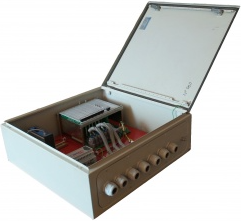
\includegraphics[width=\textwidth]{media/ict/image4}
        \caption*{DC-2 controller}
    \end{subfigure}
    \hspace{0.05\textwidth} % Adjust horizontal space between the subfigures
    \begin{subfigure}[t]{0.4\textwidth} % Align at the top
        \centering
        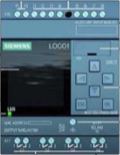
\includegraphics[width=0.7\textwidth]{media/ict/image5}
        \caption*{LOGO!230RCE}
    \end{subfigure}
        \caption*{Figure 1 - The layout of the DC-2 and the general view of the
Siemens LOGO! 230RCE microcontroller}
\end{figure}

\begin{figure}[H]
	\centering
	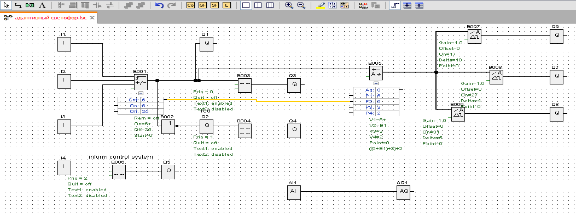
\includegraphics[width=0.8\textwidth]{media/ict/image6}
	\caption*{Figure 2 - The code of the adaptive traffic light program}
\end{figure}

\begin{multicols}{2}
The dimensions of the DC-2 and the length of the DIN rail PLC LOGO! they
are compact enough. Please note that the 230rce allows you to attach the
rail without significant structural changes. In practice, an additional
relay with the function of reprogramming and data exchange over Ethernet
networks is installed in the housing of the DC-2. An important feature
of the new hardware is the constantly expanding libraries of application
programs and software LOGO! and the presence of a simulator in Soft
Comfort. This is the personal logo of the microcontroller! The Web
editor can be supplemented with a web server, which allows you to
process network data streams, images obtained from video cameras
specific to the OOP application. Figure 2 shows the program code written
in the FBD graphical language {[}4-5{]}.

The algorithm of the traffic light with a recognition sensor located in
the traffic light zone of cars takes into account their number and if
the specified number of cars is exceeded (in our case, 15 cars), the
green light turns on{[}6{]}.

Figure 3 shows the standard program for switching on the temporary
phases of green, yellow and red light.
\end{multicols}

\begin{figure}[H]
	\centering
	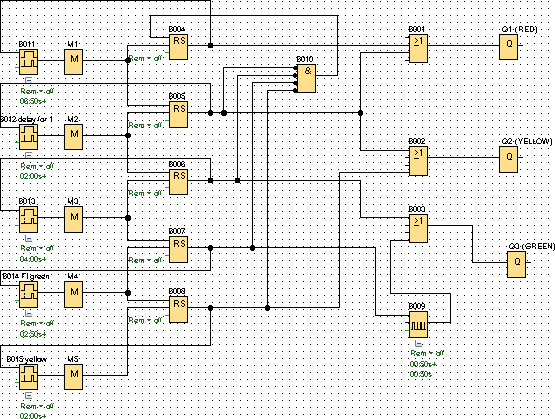
\includegraphics[width=0.8\textwidth]{media/ict/image7}
	\caption*{Figure 3 - The standard operating program of the traffic light
in the "green wave" mode}
\end{figure}

\begin{multicols}{2}
The special feature of the code is that it can be reloaded taking into
account traffic jams, emergencies and night mode (yellow, which lights
up again).

Various software solutions are used to eliminate the phenomena of
congestion and forced unreasonable delays of cars at intersections in
front of traffic lights{[}7{]}. The algorithm and Program for
calculating the number of vehicles can be adapted to a pedestrian
traffic light, which is of particular relevance for streets with divided
lanes near the centerline of the bus (for example, on Timiryazev Street
in Almaty).

In this regard, an upgraded computer traffic management system in Almaty
is needed, which should calculate online the optimal and coordinated
time intervals for switching on the phases of red, yellow, and green
traffic lights at adjacent intersections, ensuring traffic flow along
the "green" wave. Among such intelligent control systems, we note the
automated control system "Smart traffic lights" of New York City.

The intelligent traffic light control system of large cities is a
complex and expensive automated system, however, reducing travel time,
reducing vehicle downtime at intersections, reducing harmful emissions
into the atmosphere, increasing the mobility of the population as a
whole compensate for these costs. So, traffic management of a
megalopolis is a complex and multilevel technological process.

Complex automation requires a powerful computer network with central
controllers of supercomputers, on the periphery of which the IoT device
constantly transmits data to the traffic control center via
communication channels.

A promising task of modern automation of the traffic management
information system is research on "advanced" traffic management and
traffic light regulation. The implemented software products should
calculate indicators interactively, taking into account the requirements
of local government systems installed at the nodal points of the
city' s road network. Also promising tasks are the
creation of network simulators for microcontroller control of "smart
intersections", and then their localization into more complex networks
on the scale of a polycentric district and the city as a whole.
\end{multicols}

\begin{figure}[H]
	\centering
	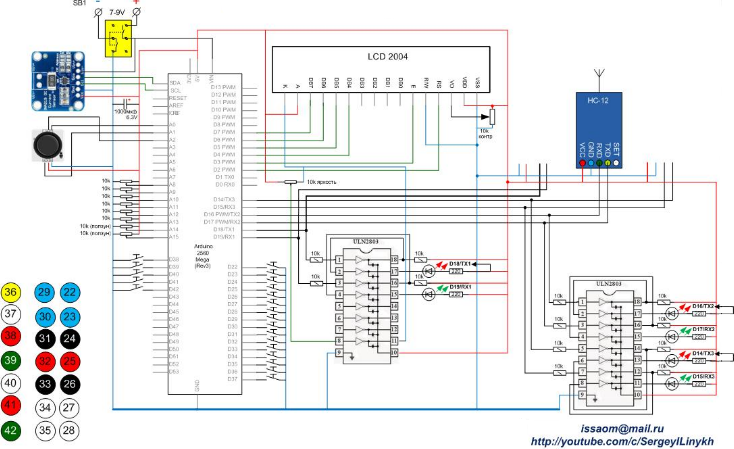
\includegraphics[width=0.9\textwidth]{media/ict/image8}
	\caption*{Figure 4 - Electrical diagram of an intelligent interface for
controlling a "smart" traffic light using a QR code}
\end{figure}

\begin{multicols}{2}
In urban conditions, the following methods of traffic management are
used:

- Control by stopping vehicles. For example, by means of traffic lights.
Each traffic flow moving through the intersection is affected by three
light signals --- green, yellow and red.

- The direction of traffic flow bypassing the area where congestion is
formed.

- Information management. The driver receives information about the
traffic situation on his way, and decides on the further route on his
own.

- Coordinated management. It allows you to increase the capacity of
roads and reduce the risk of accidents by streamlining traffic. The
following methods are used to implement coordinated management

- Rigid software control. Coordination programs and the order of their
change are calculated in advance based on movement data collected, as a
rule, by field measurements.

- Software management with forecast. The selection of the program
activation points, the duration of their operation and their adaptation
to the speed of traffic flow is performed based on data from transport
detectors.

-Adaptive control. Each cycle is implemented with the calculation of
coordination programs based on traffic flow data at each intersection
and in each control phase.

{\bfseries Results and discussions.} As a result of the conducted research,
the software and hardware of the ESP32 Cam interface was developed on
the principle of a "green wave" for special services vehicles using a QR
code. Similarly, the hardware and software of the ESP32 QR Code Reader
interface for medical vehicles was developed. The "smart" HR software
appeared during the implementation of a library program in which, with
standard QR code recognition, a text message transcribing the text of
the QR code was displayed on the screen of the COM port of the Arduino
IDE environment {[}8, 9{]} (Fig.4).


In the case of fire trucks, often driven by a small column, the "Green
Wave" has a longer turn-on time, and this information is entered into
the QR code. Below is a program that implements an algorithm for
adaptive activation of the "green wave" in the codes of the Arduino IDE
environment:
\end{multicols}

\begin{verbatim}
Void setup()
{
  TM1283 mod;
  Byte num();
  int pinA = 3;
  int pinD = 5;
  pinMode (pinA, input);
  digitalWrite(pin1);
Boolean dSW(pinC);
}
Int encoderPosCount(stepsPerrevo5){
  myStepper = 7;
  int pinDLast = 8;
  Serial.begin (362);
  Value_Y = analogRead (axis-X);
  Bool isvalid = false;
  MFRC522 mfrc522(DD_PIN;
  Byte uidCar;
  delay(1);
  mode = cloc() / 5;
  if X=4 then {
    go to 10(“.”);
    delay(100);
}
\end{verbatim}

\begin{multicols}{2}
As can be seen from the text of the application, the webcam reads the QR
code, analyzes the text and selects from it the number specified in the
text format and converts it to a digital format. Then the coil of the
intelligent traffic light relay turns on to turn on the yellow light and
then the green light.

{\bfseries Conclusion.} In conclusion, it should be noted that the
assessment of the informativeness of adaptive control algorithms makes
it possible to optimally select the necessary operating mode for traffic
flows, which in turn will significantly reduce the number of congestion
on the streets of megacities.

The use of this system has made it possible to increase the efficiency
of the automated control system by 18\%. The developed software and
hardware of the ESP32 Cam interface based on the "green wave" principle
for special services vehicles using a QR code has shown its viability
and practicality. The created program code for the Arduino IDE
environment is adapted to these requirements. The article is based on
the results of research carried out within the framework of the funded
project "A neural computer view of the smart traffic light of megacities
of the country".
\end{multicols}

\begin{center}
{\bfseries References}
\end{center}

\begin{references}
1.Badaguev B.T. Jekspluatacija transportnyh sredstv (organizacija i
bezopasnost'{} dvizhenija). -- M.:
Al' fa-Press, 2012. - 239 s. ISBN 978-5-94280-556-2 {[}in
Russian{]}

2. Dudko N.I., Petrovec V.R., Bershadskij V.F.
Bezopasnost'{} dvizhenija mehanicheskih transportnyh
sredstv: posobie - Gorki: BGSHA, 2014. - 238 s. ISBN 978-985-467-490-2
{[}in Russian{]}

3. Blinkin M.Ja. Bezopasnost'{} dorozhnogo dvizhenija:
istorija voprosa, mezhdunarodnyj opyt, bazovye institucii.-M.: Izd. dom
Vysshej shkoly jekonomiki, 2013.- 240 s. ISBN: 978-5-7598-1086-5 {[}in
Russian{]}

4. Volkov V.S. Jelektrooborudovanie transportnyh i
transportno-tehnologicheskih mashin: uchebnoe posobie - M.: Akademija,
2010. - 208 s. ISBN 978-5-7695-5749-1 {[}in Russian{]}

5. Gorev, A. Je.Osnovy teorii transportnyh sistem: uchebnoe posobie / A.
Je. Gorev;SPbGASU. -- SPb., 2010. - 214 s. ISBN 978-5-9227-0266-9 {[}in
Russian{]}

6. Majboroda M.E., Bednarskij V.V. Gruzovye
avtomobil' nye perevozki. - M.: Feniks, 2008.- 442 s.
ISBN 978-5-222-14364-3 {[}in Russian{]}

7. Klinkovshtejn G.I. Organizacija dorozhnogo dvizhenija: uchebnik dlja
vuzov. -- 5-e izd., pererab. i dop.- M: Transport, 2001 - 247. ISBN
9785277022405

8. Urykov V.A., Zelenina L.I. Modeli transportnogo infrastrukturnogo
kompleksa //
\href{https://web.snauka.ru/issues/2014.\%2018.06.2020}{https://web.snauka.ru}. {[}in Russian{]}

9. Morozov I.I. i dr. Chislennoe issledovanie transportnyh potokov na
osnove gidrodinamicheskih modelej // Komp' juternye
issledovanija i modelirovanie.-2011. -T. 3(4).-S. 389-412. {[}in
Russian{]}
\end{references}

\begin{authorinfo}
\hspace{1em}\emph{{\bfseries Сведения об авторах}}

Тулегулов А.Д. - кандидат физико-математических наук, ассоциированный
профессор, Казахский университет технологии и бизнеса имени К.
Кулажанова, Астана, Казахстан, e-mail: tad62@ya.ru;

Акишев К.М. - кандидат технических наук, ассоциированный профессор,
Казахский университет технологии и бизнеса имени К. Кулажанова, Астана,
Казахстан, e-mail: akmail04@ya.ru;

Жамангарин Д. С.- PhD, Казахский университет технологии и бизнеса имени
К. Кулажанова, Астана, Казахстан, е-mail:
\href{mailto:Dus_man89@mail.ru}{\nolinkurl{Dus\_man89@mail.ru}};

Юрков Н.К. - доктор технических наук, профессор, Пензенский
государственный университет, Пенза, Россия, е-mail:
\href{mailto:kipra@mail.ru}{\nolinkurl{kipra@mail.ru}};

Акишева Л.К.-исследователь, Назарбаев интеллектуальная школа, Астана,
Казахстан, е-mail: akmail04@ya.ru

Алтынбек С. А. {\bfseries -} PhD, ассоциированный профессор, Казахский
университет технологии и бизнеса, Астана, Казахстан, е-mail:
\href{mailto:serik_aa@bk.ru}{\nolinkurl{serik\_aa@bk.ru}};

Смакова Н.С. - PhD, ассоциированный профессор, Казахский университет
технологии и бизнеса, Астана, Казахстан, е-mail:nuri\_5@mail.ru

\hspace{1em}\emph{{\bfseries Information about the authors}}

Tulegulov A.D. - Candidate of Physical and Mathematical Sciences,
Associate Professor, Kazakh University of Technology and Business named
after K. Kulazhanov, Astana, Kazakhstan, e-mail:
\href{mailto:tad62@ya.ru}{\nolinkurl{tad62@ya.ru}};

Akishev K.M. - Candidate of Technical Sciences, Associate Professor,
Kazakh University of Technology and Business named after K. Kulazhanov,
Astana, Kazakhstan, e-mail:
\href{mailto:akmail04@ya.ru}{\nolinkurl{akmail04@ya.ru}};

Zhamangarin D. S.- PhD, K. Kulazhanov Kazakh University of Technology
and Business, Astana, Kazakhstan,

e-mail: \href{mailto:Dus_man89@mail.ru}{\nolinkurl{Dus\_man89@mail.ru}};

Akisheva L.K.-researcher, Nazarbayev Intellectual School, Astana,
Kazakhstan, e-mail: akmail04@ya.ru

Yurkov N.K. - Doctor of Technical Sciences, Professor, Penza State
University, Penza, Russia, е-mail:
\href{mailto:kipra@mail.ru}{\nolinkurl{kipra@mail.ru}};

Altynbek S. A. PhD, Associate Professor, Kazakh University of Technology
and Business, Astana, Kazakhstan, е-mail:

\href{mailto:serik_aa@bk.ru}{\nolinkurl{serik\_aa@bk.ru}}

Smakova N.S.- PhD, Associate Professor, Kazakh University of Technology
and Business, Astana, Kazakhstan, е-mail: \\\href{mailto:nuri\_5@mail.ru}{\nolinkurl{nuri\_5@mail.ru}}
\end{authorinfo}
